\documentclass{article}
\usepackage{pgfplots}
\pgfplotsset{compat=1.18}

\begin{document}

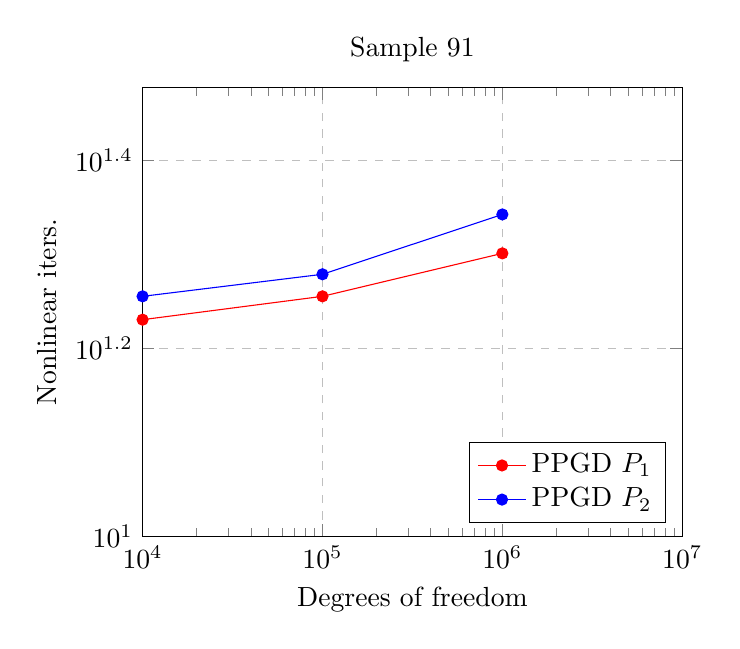
\begin{tikzpicture}
    \begin{loglogaxis}[
        xlabel={Degrees of freedom},
        ylabel={Nonlinear iters.},
        legend pos=south east,
        legend cell align=left,
        log basis x={10},
        log basis y={10},
        ymin=10,
        ymax=30,
        xmin=1e4,
        xmax=1e7,
        grid=major,
        grid style=dashed,
        tick label style={/pgf/number format/fixed},
        title style={align=center},
        title={Sample 91},
        ]
        \addplot[red, mark=*] coordinates {
            (1e4, 17)
            (1e5, 18)
            (1e6, 20)
        };
        \addlegendentry{PPGD $\mathbb{P}_1$}
        
        \addplot[blue, mark=*] coordinates {
            (1e4, 18)
            (1e5, 19)
            (1e6, 22)
        };
        \addlegendentry{PPGD $\mathbb{P}_2$}
    \end{loglogaxis}
\end{tikzpicture}

\end{document}